\documentclass[tikz,border=4pt]{standalone}
\usepackage{amsmath,amssymb}
\usetikzlibrary{arrows.meta,calc}
\begin{document}
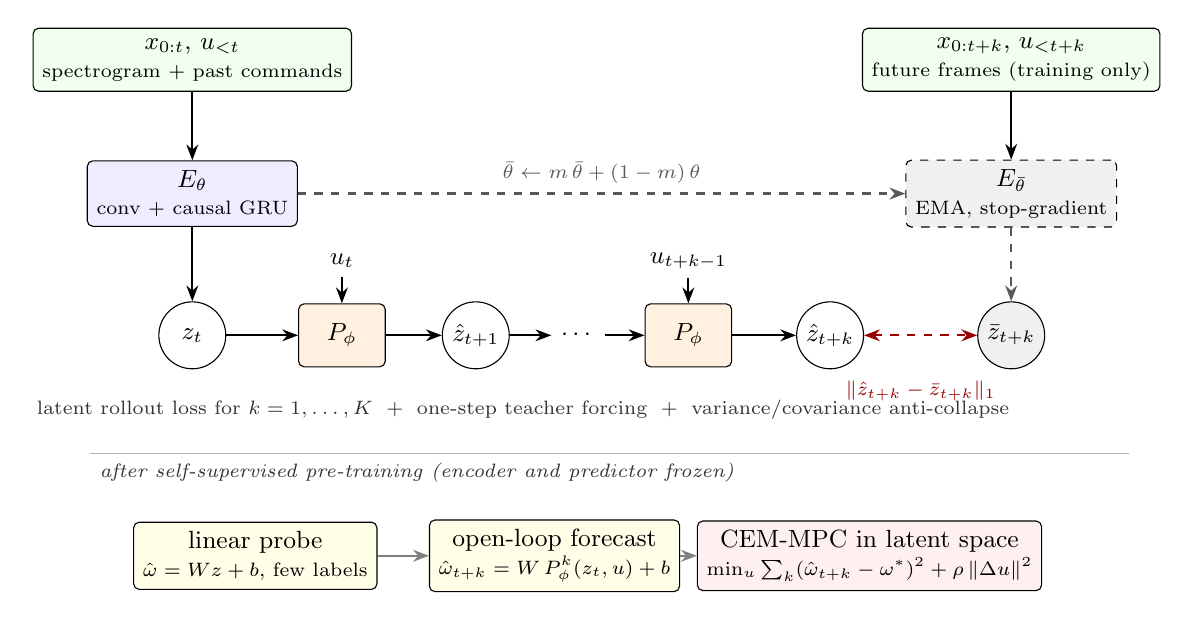
\begin{tikzpicture}[
  font=\small,
  box/.style={draw, rounded corners=2pt, minimum height=8mm, minimum width=18mm, align=center, fill=white},
  enc/.style={box, fill=blue!7},
  tgt/.style={box, fill=gray!12, dashed},
  pred/.style={box, fill=orange!12, minimum width=11mm},
  lat/.style={circle, draw, inner sep=0.5pt, minimum size=8.5mm, fill=white},
  arr/.style={-{Stealth[length=2mm]}, thick},
  sg/.style={-{Stealth[length=2mm]}, thick, dashed, gray!70!black},
]
% Observations and encoders
\node[box, fill=green!6] (x0) at (0,0) {$x_{0:t},\,u_{<t}$\\[-1pt]\scriptsize spectrogram + past commands};
\node[box, fill=green!6] (xk) at (10.4,0) {$x_{0:t+k},\,u_{<t+k}$\\[-1pt]\scriptsize future frames (training only)};
\node[enc] (E) at (0,-1.7) {$E_\theta$\\[-1pt]\scriptsize conv + causal GRU};
\node[tgt] (Eb) at (10.4,-1.7) {$E_{\bar\theta}$\\[-1pt]\scriptsize EMA, stop-gradient};
\draw[arr] (x0) -- (E);
\draw[arr] (xk) -- (Eb);
\draw[sg] (E.east) -- node[above, font=\scriptsize] {$\bar\theta \leftarrow m\,\bar\theta + (1-m)\,\theta$} (Eb.west);
% Latent rollout
\node[lat] (zt) at (0,-3.5) {$z_t$};
\node[pred] (P1) at (1.9,-3.5) {$P_\phi$};
\node[lat] (z1) at (3.6,-3.5) {$\hat z_{t+1}$};
\node (dots) at (4.9,-3.5) {$\cdots$};
\node[pred] (Pk) at (6.3,-3.5) {$P_\phi$};
\node[lat] (zk) at (8.1,-3.5) {$\hat z_{t+k}$};
\node[lat, fill=gray!12] (zb) at (10.4,-3.5) {$\bar z_{t+k}$};
\node (u0) at (1.9,-2.55) {$u_t$};
\node (uk) at (6.3,-2.55) {$u_{t+k-1}$};
\draw[arr] (E) -- (zt);
\draw[arr] (zt) -- (P1); \draw[arr] (P1) -- (z1); \draw[arr] (z1) -- (dots); \draw[arr] (dots) -- (Pk); \draw[arr] (Pk) -- (zk);
\draw[arr] (u0) -- (P1); \draw[arr] (uk) -- (Pk);
\draw[sg] (Eb) -- (zb);
\draw[thick, dashed, red!60!black, <->, >={Stealth[length=2mm]}] (zk) -- node[below=4.5mm, font=\scriptsize, text=red!60!black] {$\|\hat z_{t+k}-\bar z_{t+k}\|_1$} (zb);
\node[font=\scriptsize, align=center, text=gray!40!black] at (4.2,-4.45)
  {latent rollout loss for $k=1,\dots,K$ \;+\; one-step teacher forcing \;+\; variance/covariance anti-collapse};
% Downstream use
\draw[gray!60, thin] (-1.3,-5.0) -- (11.9,-5.0);
\node[font=\scriptsize\itshape, anchor=west, text=gray!40!black] at (-1.3,-5.25) {after self-supervised pre-training (encoder and predictor frozen)};
\node[box, fill=yellow!10] (probe) at (0.8,-6.3) {linear probe\\[-1pt]\scriptsize $\hat\omega = W z + b$, few labels};
\node[box, fill=yellow!10] (roll) at (4.6,-6.3) {open-loop forecast\\[-1pt]\scriptsize $\hat\omega_{t+k} = W\,P_\phi^{k}(z_t,u)+b$};
\node[box, fill=red!6] (mpc) at (8.6,-6.3) {CEM-MPC in latent space\\[-1pt]\scriptsize $\min_u \sum_k (\hat\omega_{t+k}-\omega^\ast)^2 + \rho\,\|\Delta u\|^2$};
\draw[arr, gray] (probe) -- (roll); \draw[arr, gray] (roll) -- (mpc);
\end{tikzpicture}
\end{document}
